\begin{appendices}
	\section*{Imágenes de algunas anomalías en la carretera}
		\begin{figure}[htb]
			  \centering
			  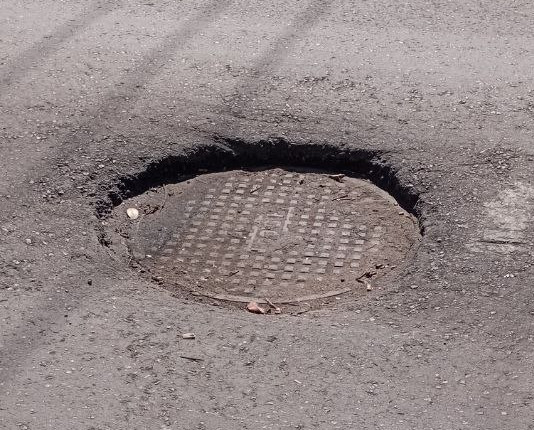
\includegraphics[scale = 0.4]{Graphics/pothole_3.jpg}
			  \caption{Boca de alcantarilla hundida en el pavimento}
			  \label{fig:15}
		\end{figure}

		\begin{figure}[htb]
			  \centering
			  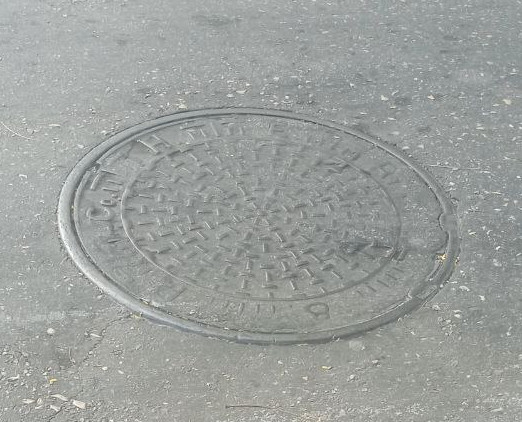
\includegraphics[scale = 0.4]{Graphics/pothole_9.jpg}
			  \caption{Boca de alcantarilla}
			  \label{fig:16}
		\end{figure}
		\newpage

		\begin{figure}[htb]
			\centering
			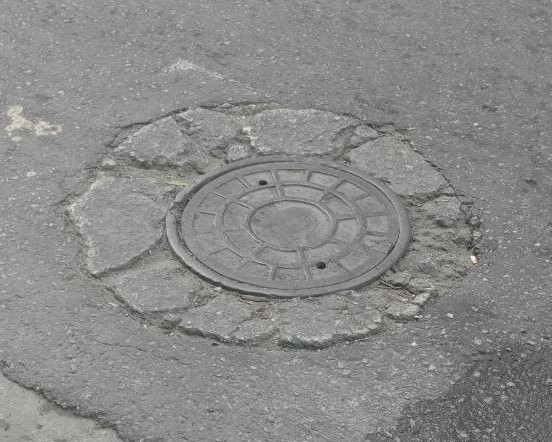
\includegraphics[scale = 0.3]{Graphics/pothole_4.jpg}
			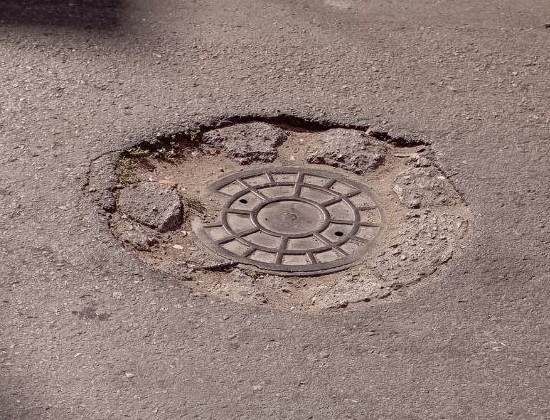
\includegraphics[scale = 0.3]{Graphics/pothole_5.jpg}
			\caption{tapas de alcantarilla con características anormales}
			\label{fig:17}
		\end{figure}
		\newpage

		\begin{figure}[htb]
			\centering
			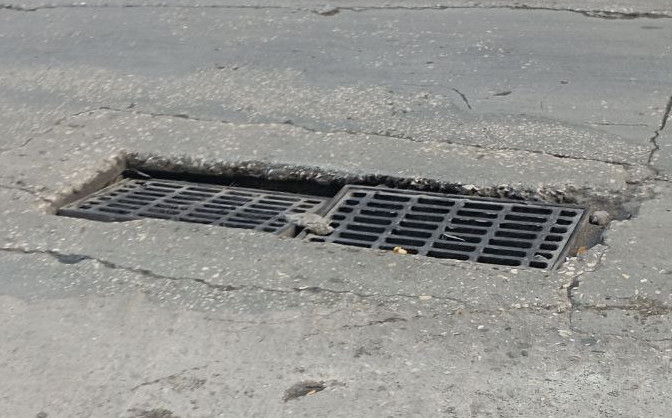
\includegraphics[scale = 0.3]{Graphics/pothole_10.jpg}
			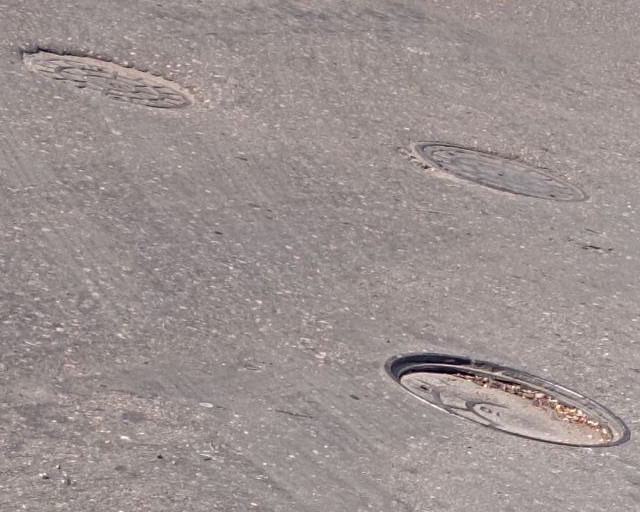
\includegraphics[scale = 0.3]{Graphics/pothole_11.jpg}
			\caption{Otros objetos en la vía con características anormales}
			\label{fig:18}
		\end{figure}

		\begin{figure}[htb]
			\centering
			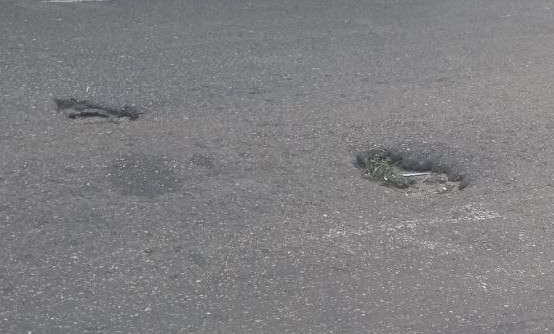
\includegraphics[scale = 0.3]{Graphics/pothole_7.jpg}
			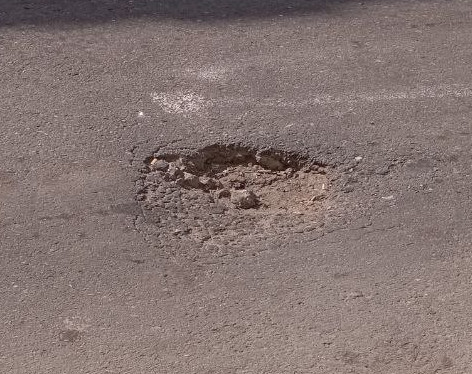
\includegraphics[scale = 0.3]{Graphics/pothole_8.jpg}
			\caption{Algunos baches de algunas de las rutas seleccionadas}
			\label{fig:19}
		\end{figure}

		\newpage
		\begin{figure}[htb]
			\centering
			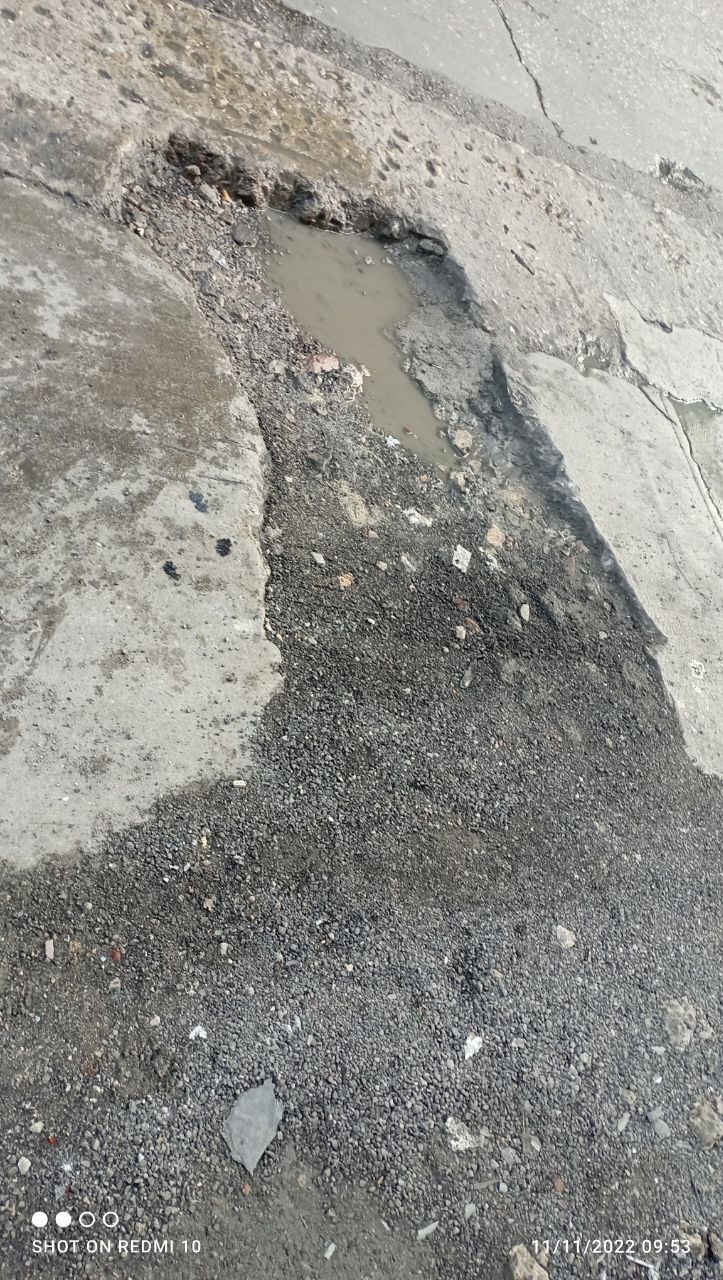
\includegraphics[scale = 0.3]{Graphics/pothole_1.jpg}
			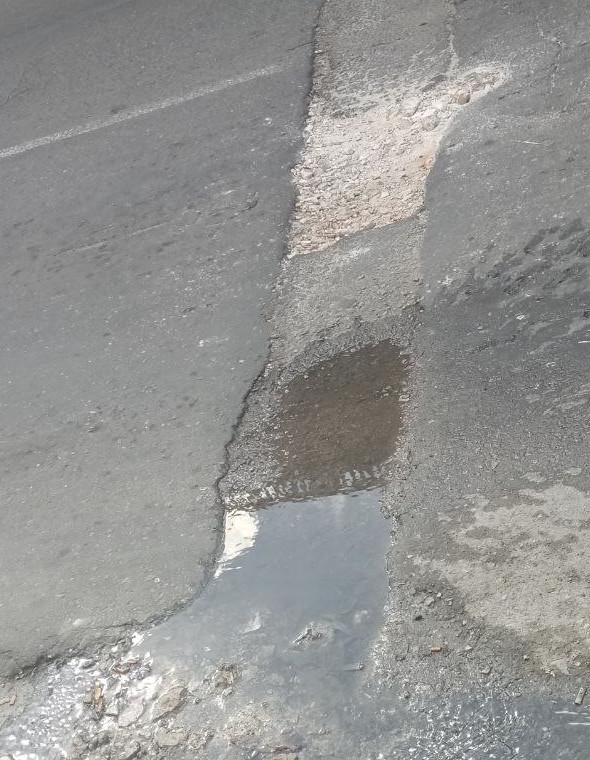
\includegraphics[scale = 0.3]{Graphics/pothole_2.jpg}
			\caption{Más baches de algunas de las rutas seleccionadas}
			\label{fig:20}
		\end{figure}
		\newpage

	\section*{Tablas con los hiperparámetros que se probaron los métodos de detección de anomalías no-supervisados}

		\begin{table}[htb]
			\centering
			\caption{Hiperparámetros con los que se probó \textbf{DBSCAN}}
			\label{table:4}
			\begin{tabular}{lc}
			\toprule
			Hiperparámetro &                                     Valores \\
			\midrule
					   eps & 0.05, 0.1, 0.15, 0.20, ... 0.90, 0.95, 0.99 \\
			   min\_samples & 15, 20, 25, 30, 25, 40,  45, 50, 55, 60, 65 \\
			\bottomrule
			\end{tabular}
		\end{table}

		\begin{table}[htb]
			\centering
			\caption{Hiperparámetros con los que se probó \textbf{One Class SVM}}
			\label{table:5}
			\begin{tabular}{lc}
			\toprule
			Hiperparámetro &                                            Valores \\
			\midrule
					 gamma &    scale, 0.00001, 0.0001, 0.001, 0.01, 0.1, 1, 10 \\
						nu & 0.05, 0.15, 0.2 ..., 0.8, 0.85, 0.95, 0.99 \\
			\bottomrule
			\end{tabular}
		\end{table}
		
		\begin{table}[htb]
			\centering
			\caption{Hiperparámetros con los que se probó \textbf{OPTICS}}
			\label{table:6}
			\begin{tabular}{lc}
			\toprule
			Hiperparámetro &                                           Valores \\
			\midrule
			cluster\_method &                                        xi, dbscan \\
					metric &        minkowski, euclidean, canberra, braycurtis \\
			   min\_samples & 5, 10, 15, 20, 25, 30, 35, 40, 45, 50, 55, 60, 65 \\
			\bottomrule
			\end{tabular}
		\end{table}
		
	\newpage
	\section*{Tablas con los hiperparámetros que se probaron los métodos supervisados}

		\begin{table}[ht!]
			\centering
			\caption{Hiperparámetros con los que se probó  \textbf{KNN}}
			\label{table:7}
			\begin{tabular}{lc}
				\toprule
				Hiperparámetro &                   Valores \\
				\midrule
				   n\_neighbors &            3, 5, 7, 9, 11 \\
					   weights &         uniform, distance \\
					 algorithm & brute, kd\_tree, ball\_tree \\
					 leaf\_size &            20, 30, 40, 50 \\
				\bottomrule
			\end{tabular}
		\end{table}

		\begin{table}[ht!]
			\centering
			\caption{Hiperparámetros con los que se probó \textbf{\emph{Decision Tree}}}
			\label{table:8}
			\begin{tabular}{lc}
				\toprule
				Hiperparámetro &          Valores \\
				\midrule
				     criterion &    entropy, gini \\
				      splitter &     best, random \\
				     max\_depth & 3, 4, 5, 6, None \\
				  max\_features & sqrt, log2, None \\
				\bottomrule
			\end{tabular}
		\end{table}

		\begin{table}[ht!]
			\centering
			\caption{Hiperparámetros con los que se probó \textbf{\emph{Random Forest}}}
			\label{table:9}
			\begin{tabular}{lc}
				\toprule
				Hiperparámetro &         Valores \\
				\midrule
				  n\_estimators &   100, 120, 180 \\
					 criterion &   entropy, gini \\
					 max\_depth & 10,  13, 16, 20 \\
				  max\_features &      log2, sqrt \\
				\bottomrule
			\end{tabular}
		\end{table}
			
		

		\begin{table}[ht!]
			\centering
			\caption{Hiperparámetros con los que se probó \textbf{Regresión Logística}}
			\label{table:10}
			\begin{tabular}{lc}
				\toprule
				Hiperparámetro &                Valores \\
				\midrule
					   penalty &                     l2 \\
						   tol & 1e-3, 1e-4, 1e-5, 1e-6 \\
							 C &       1, 10, 100, 1000 \\
						solver &            lbfgs, saga \\
					  max\_iter &         100, 500, 1000 \\
				\bottomrule
			\end{tabular}
		\end{table}
		
		
		\begin{table}[htb]
			\centering
			\caption{Hiperparámetros con los que se probó \textbf{SVM}}
			\label{table:11}
			\begin{tabular}{lc}
			\toprule
			Hiperparámetro &                           Valores \\
			\midrule
						 C &              1, 10, 50, 100, 1000 \\
					kernel &                               rbf \\
					 gamma & 0.1, 0.01, 0.001, 0.0001, 0.00001 \\
			   probability &                              True \\
			\bottomrule
			\end{tabular}
		\end{table}

	\newpage
	\section*{Las características más seleccionadas}
		\begin{table}[htb]
			\centering
			\caption{Las 10 características más seleccionadas}
			\label{table:12}
				\begin{tabular}{lc}
				\toprule
						Feature &  Count \\
				\midrule
						  X / Z &    203 \\
					   SpeedvsZ &    185 \\
				   MeanDevGyroZ &    180 \\
				 MedianDevGyroZ &    164 \\
					  MinZratio &    145 \\
						 Z Gyro &    136 \\
						 Y Gyro &    132 \\
				MedianDevAccelY &    132 \\
						 X Gyro &    125 \\
				 MedianDevGyroY &    119 \\
				\bottomrule
				\end{tabular}
		\end{table}
	
	\section*{Mejores resultados e hiperparámetros seleccionados}
		\begin{table}[htb]
			\centering
			\caption{Mejor resultado obtenido con \textbf{Z-Thresh} y \textbf{KNN}}
			\label{table:17}
			\begin{tabular}{lc}
				\toprule
					  Método de detección de anomalías &                                         z\_thresh \\
				Método de selección de características &                               backward\_selection \\
						 Características seleccionadas & \{MeanDevAccelY, MedianDevAccelZ,    \\
						 							   &									MedianDevGyroY\} \\
												modelo &                                              KNN \\
											  F1 score &                                         0.470588 \\
											 Precision &                                              0.5 \\
												Recall &                                         0.444444 \\
											  Accuracy &                                         0.689655 \\
				\bottomrule
			\end{tabular}
			\newline
			\newline

			\begin{tabular}{lc}
				\toprule
				Hiperparámetro &    Valor \\
				\midrule
					 algorithm &  kd\_tree \\
					 leaf\_size &       50 \\
				   n\_neighbors &        3 \\
					   weights & distance \\
				\bottomrule
			\end{tabular}
			
			
		\end{table}

		\begin{table}[htb]
			\centering
			\caption{Mejor resultado obtenido con \textbf{Z-Diff} y \textbf{KNN}}
			\label{table:18}
			\begin{tabular}{lc}
				\toprule
					  Método de detección de anomalías &                                     z\_diff \\
				Método de selección de características &                         backward\_selection \\
						 Características seleccionadas & \{MeanDevGyroX, MeanDevGyroY, \\
						 							   & 							MeanDevGyroZ\}   \\
												modelo &                                        KNN \\
											  F1 score &                                        0.5 \\
											 Precision &                                   0.583333 \\
												Recall &                                     0.4375 \\
											  Accuracy &                                   0.745455 \\
				\bottomrule
			\end{tabular}
			\newline
			\newline

			\begin{tabular}{lc}
				\toprule
				Hiperparámetro &     Valor \\
				\midrule
					 algorithm & ball\_tree \\
					 leaf\_size &        40 \\
				   n\_neighbors &         5 \\
					   weights &  distance \\
				\bottomrule
			\end{tabular}
			
		\end{table}

		\begin{table}[htb]
			\caption{Mejor resultado obtenido con \textbf{DBSCAN} y \textbf{KNN}}
			\label{table:19}
			\centering
			\begin{tabular}{lc}
				\toprule
				      Método de detección de anomalías &                                 dbscan \\
				Método de selección de características &                     backward\_selection \\
				         Características seleccionadas & \{X / Z, MedianDevAccelY,               \\
						 							   &                   MeanDevGyroZ\} \\
				                                modelo &                                    KNN \\
				                              F1 score &                                    0.6 \\
				                             Precision &                                    0.6 \\
				                                Recall &                                    0.6 \\
				                              Accuracy &                               0.707317 \\
				\bottomrule
			\end{tabular}
			\newline
			\newline

			\begin{tabular}{lc}
				\toprule
				Hiperparámetro &    Valor \\
				\midrule
					 algorithm &  kd\_tree \\
					 leaf\_size &       50 \\
				   n\_neighbors &        3 \\
					   weights & distance \\
				\bottomrule
			\end{tabular}
			
			
		\end{table}

		\begin{table}[htb]
			\centering
			\caption{Mejor resultado obtenido con \textbf{One Class SVM} y \textbf{KNN}}
			\label{table:20}
			\begin{tabular}{lc}
				\toprule
					  Método de detección de anomalías &                                              ocsvm \\
				Método de selección de características &                                 backward\_selection \\
						 Características seleccionadas & 					\{Y Accel, X Gyro, Z Gyro, X / Z, \\
						 							   &	MeanDevAccelZ, MedianDevGyroX, MedianDevGyroY,   \\
													   &	MeanDevGyroZ, MedianDevGyroZ\} \\
												modelo &                                                KNN \\
											  F1 score &                                            0.42623 \\
											 Precision &                                           0.565217 \\
												Recall &                                           0.342105 \\
											  Accuracy &                                           0.738806 \\
				\bottomrule
			\end{tabular}
			\newline
			\newline

			\begin{tabular}{lc}
				\toprule
				Hiperparámetro &    Valor \\
				\midrule
					 algorithm &  kd\_tree \\
					 leaf\_size &       50 \\
				   n\_neighbors &        3 \\
					   weights & distance \\
				\bottomrule
			\end{tabular}
			
		\end{table}
	
		\begin{table}[htb]
			\centering
			\caption{Mejor resultado obtenido con \textbf{Z-Thresh} y \textbf{\emph{Decision Tree}}}
			\label{table:21}
			\begin{tabular}{lc}
				\toprule
					  Método de detección de anomalías &                          z\_thresh \\
				Método de selección de características &                 forward\_selection \\
						 Características seleccionadas & \{Y Accel, Z Gyro, MedianDevGyroX \} \\
												modelo &                     Decision Tree \\
											  F1 score &                               0.4 \\
											 Precision &                          0.363636 \\
												Recall &                          0.444444 \\
											  Accuracy &                          0.586207 \\
				\bottomrule
				\end{tabular}
			\newline
			\newline

			\begin{tabular}{lc}
				\toprule
				Hiperparámetro & Valor \\
				\midrule
					 criterion &  gini \\
					 max\_depth &  None \\
				  max\_features &  log2 \\
					  splitter &  best \\
				\bottomrule
			\end{tabular}
			
		\end{table}

		\begin{table}[htb]
			\centering
			\caption{Mejor resultado obtenido con \textbf{Z-Diff} y \textbf{\emph{Decision Tree}}}
			\label{table:22}
			\begin{tabular}{lc}
				\toprule
					  Método de detección de anomalías &                                   z\_diff \\
				Método de selección de características &                    recursive\_elimination \\
						 Características seleccionadas & \{SpeedvsZ, MedianDevGyroY, MeanDevGyroZ\}\\
												modelo &                            Decision Tree \\
											  F1 score &                                      0.5 \\
											 Precision &                                 0.392857 \\
												Recall &                                   0.6875 \\
											  Accuracy &                                      0.6 \\
				\bottomrule
				\end{tabular}
			\newline
			\newline

			\begin{tabular}{lc}
				\toprule
				Hiperparámetro & Valor \\
				\midrule
					 criterion &  gini \\
					 max\_depth &  None \\
				  max\_features &  None \\
					  splitter &  best \\
				\bottomrule
			\end{tabular}
			
		\end{table}

		\begin{table}[htb]
			\centering
			\caption{Mejor resultado obtenido con \textbf{DBSCAN} y \textbf{\emph{Decision Tree}}}
			\label{table:23}
			\begin{tabular}{lc}
				\toprule
					  Método de detección de anomalías &                                             dbscan \\
				Método de selección de características &                                  forward\_selection \\
						 Características seleccionadas & \{X Accel, Z Gyro, X / Z, MinZratio, SpeedvsZ, \\
						 							   &   MeanDevAccelX, MeanDevAccelY, MedianDevAccelY, \\
													   &                                    MeanDevGyroZ \} \\
												modelo &                                      Decision Tree \\
											  F1 score &                                           0.628571 \\
											 Precision &                                               0.55 \\
												Recall &                                           0.733333 \\
											  Accuracy &                                           0.682927 \\
				\bottomrule
			\end{tabular}
			\newline
			\newline

			\begin{tabular}{lc}
				\toprule
				Hiperparámetro &   Valor \\
				\midrule
					 criterion & entropy \\
					 max\_depth &    None \\
				  max\_features &    log2 \\
					  splitter &    best \\
				\bottomrule
			\end{tabular}
			
		\end{table}

		\begin{table}[htb]
			\centering
			\caption{Mejor resultado obtenido con \textbf{One Class SVM} y \textbf{\emph{Decision Tree}}}
			\label{table:24}
			\begin{tabular}{lc}
				\toprule
					  Método de detección de anomalías &                                              ocsvm \\
				Método de selección de características &                              recursive\_elimination \\
						 Características seleccionadas & \{Y Gyro, X / Z, MaxZratio, MinZratio, \\
						 							   &   SpeedvsZ,  MeanDevAccelY \}\\
												modelo &                                      Decision Tree \\
											  F1 score &                                           0.394366 \\
											 Precision &                                           0.424242 \\
												Recall &                                           0.368421 \\
											  Accuracy &                                           0.679104 \\
				\bottomrule
			\end{tabular}
			\newline
			\newline

			\begin{tabular}{lc}
				\toprule
				Hiperparámetro &   Valor \\
				\midrule
					 criterion & entropy \\
					 max\_depth &    None \\
				  max\_features &    sqrt \\
					  splitter &    best \\
				\bottomrule
			\end{tabular}
			
		\end{table}

		\begin{table}[htb]
			\caption{Mejor resultado obtenido con \textbf{Z-Thresh} y \textbf{SVM}}
			\label{table:25}
			\centering
			\begin{tabular}{lc}
				\toprule
					  Método de detección de anomalías &                                         z\_thresh \\
				Método de selección de características &                               backward\_selection  \\
						 Características seleccionadas & \{MeanDevAccelY, MedianDevAccelZ,  \\
						 							   &                                MedianDevGyroY\}  \\
												modelo &                                              SVM  \\
											  F1 score &                                         0.470588 \\
											 Precision &                                              0.5 \\
												Recall &                                         0.444444 \\
											  Accuracy &                                         0.689655 \\
				\bottomrule
			\end{tabular}
			\newline
			\newline

			\begin{tabular}{lc}
				\toprule
				Hiperparámetro & Valor \\
				\midrule
							 C &  1000 \\
						 gamma &   0.1 \\
						kernel &   rbf \\
				   probability &  true \\
				\bottomrule
			\end{tabular}
			
		\end{table}

		\begin{table}[htb]
			\centering
			\caption{Mejor resultado obtenido con \textbf{Z-Diff} y \textbf{SVM}}
			\label{table:26}
			\begin{tabular}{lc}
				\toprule
					  Método de detección de anomalías &                                             z\_diff \\
				Método de selección de características &                                 backward\_selection \\
						 Características seleccionadas & \{X Gyro, Z Gyro, SpeedvsZ, MeanDevGyroX, \\
						 							   &      MeanDevGyroY, MedianDevGyroY \} \\
												modelo &                                                SVM \\
											  F1 score &                                                0.5 \\
											 Precision &                                                0.5 \\
												Recall &                                                0.5 \\
											  Accuracy &                                           0.709091 \\
				\bottomrule
				\end{tabular}
			\newline
			\newline

			\begin{tabular}{lc}
			\toprule
			Hiperparámetro & Valor \\
			\midrule
						 C &  1000 \\
					 gamma &   0.1 \\
					kernel &   rbf \\
			   probability &  true \\
			\bottomrule
			\end{tabular}
			
		\end{table}

		\begin{table}[htb]
			\centering
			\caption{Mejor resultado obtenido con \textbf{DBSCAN} y \textbf{SVM}}
			\label{table:27}

			\begin{tabular}{lc}
				\toprule
					  Método de detección de anomalías &                                             dbscan \\
				Método de selección de características &                                  forward\_selection \\
						 Características seleccionadas & \{X Accel, X Gyro, X / Z \\
						 							   &  MinZratio, MedianDevAccelY, MeanDevGyroZ \} \\
												modelo &                                                SVM \\
											  F1 score &                                           0.684211 \\
											 Precision &                                           0.565217 \\
												Recall &                                           0.866667 \\
											  Accuracy &                                           0.707317 \\
				\bottomrule
			\end{tabular}
			\newline
			\newline

			\begin{tabular}{lc}
				\toprule
				Hiperparámetro & Valor \\
				\midrule
							 C &    50 \\
						 gamma &   0.1 \\
						kernel &   rbf \\
				   probability &  true \\
				\bottomrule
			\end{tabular}
			
		\end{table}

		\begin{table}[htb]
			\centering
			\caption{Mejor resultado obtenido con \textbf{One Class SVM} y \textbf{SVM}}
			\label{table:28}
			\begin{tabular}{lc}
				\toprule
					  Método de detección de anomalías &                                              ocsvm \\
				Método de selección de características &                              recursive\_elimination \\
						 Características seleccionadas & \{Y Gyro, X / Z, MinZratio, SpeedvsZ,   \\ 
						 							   &   MeanDevAccelX, MeanDevGyroX \}\\
												modelo &                                                SVM \\
											  F1 score &                                           0.366197 \\
											 Precision &                                           0.393939 \\
												Recall &                                           0.342105 \\
											  Accuracy &                                           0.664179 \\
				\bottomrule
			\end{tabular}
			\newline
			\newline

			\begin{tabular}{lc}
				\toprule
				Hiperparámetro & Valor \\
				\midrule
							 C &  1000 \\
						 gamma &   0.1 \\
						kernel &   rbf \\
				   probability &  true \\
				\bottomrule
			\end{tabular}
			
		\end{table}

		\begin{table}[htb]
			\centering
			\caption{Mejor resultado obtenido con \textbf{Z-Thresh} y \textbf{Regresión Logística}}
			\label{table:29}
			\begin{tabular}{lc}
				\toprule
					  Método de detección de anomalías &                                           z\_thresh \\
				Método de selección de características &                                 backward\_selection \\
						 Características seleccionadas & \{MedianDevAccelX, MeanDevAccelY, \\ 
						                               &  MedianDevAccelZ, MeanDevGyroX, \\
						 							   &    ,MedianDevGyroX, MeanDevGyroY \}\\		
												modelo &                                     Log Regression \\
											  F1 score &                                                0.2 \\
											 Precision &                                                1.0 \\
												Recall &                                           0.111111 \\
											  Accuracy &                                           0.724138 \\
				\bottomrule
			\end{tabular}
			\newline
			\newline

			\begin{tabular}{lc}
				\toprule
				Hiperparámetro &     Valor \\
				\midrule
							 C &        10 \\
					  max\_iter &       100 \\
					   penalty &        l2 \\
						solver &      saga \\
						   tol &  0.000001 \\
				\bottomrule
			\end{tabular}
			
		\end{table}

		\begin{table}[htb]
			\centering
			\caption{Mejor resultado obtenido con \textbf{Z-Diff} y \textbf{Regresión Logística}}
			\label{table:30}
			\begin{tabular}{lc}
				\toprule
					  Método de detección de anomalías &                              z\_diff \\
				Método de selección de características &               recursive\_elimination \\
						 Características seleccionadas & \{Y Gyro, MinZratio, MedianDevGyroZ\} \\
												modelo &                      Log Regression \\
											  F1 score &                                0.32 \\
											 Precision &                            0.444444 \\
												Recall &                                0.25 \\
											  Accuracy &                            0.690909 \\
				\bottomrule
				\end{tabular}
			\newline
			\newline

			\begin{tabular}{lc}
				\toprule
				Hiperparámetro &  Valor \\
				\midrule
							 C &    100 \\
					  max\_iter &   1000 \\
					   penalty &     l2 \\
						solver &   saga \\
						   tol &  0.001 \\
				\bottomrule
			\end{tabular}
			
		\end{table}

		\begin{table}[htb]
			\centering
			\caption{Mejor resultado obtenido con \textbf{DBSCAN} y \textbf{Regresión Logística}}
			\label{table:31}
			\begin{tabular}{lc}
				\toprule
					  Método de detección de anomalías &                                             dbscan \\
				Método de selección de características &                              recursive\_elimination \\
						 Características seleccionadas & \{X Accel, Y Accel, Y Gyro, Z Gyro, X / Z, \\ 
						 							   &    MinZratio, SpeedvsZ, MeanDevAccelY,\\
													   &  MedianDevGyroZ \} \\
												modelo &                                     Log Regression \\
											  F1 score &                                                0.5 \\
											 Precision &                                           0.666667 \\
												Recall &                                                0.4 \\
											  Accuracy &                                           0.707317 \\
				\bottomrule
				\end{tabular}
			\newline
			\newline

			\begin{tabular}{lc}
				\toprule
				Hiperparámetro &     Valor \\
				\midrule
							 C &       100 \\
					  max\_iter &      1000 \\
					   penalty &        l2 \\
						solver &      saga \\
						   tol &  0.000001 \\
				\bottomrule
			\end{tabular}
			
		\end{table}

		\begin{table}[htb]
			\centering
			\caption{Mejor resultado obtenido con \textbf{One Class SVM} y \textbf{Regresión Logística}}
			\label{table:32}
			\begin{tabular}{lc}
				\toprule
					  Método de detección de anomalías &                                              ocsvm \\
				Método de selección de características &                              recursive\_elimination \\
						 Características seleccionadas & \{Y Accel, X Gyro, Y Gyro, Z Gyro, \\ 
						 							   &  X / Z,  MinZratio, SpeedvsZ, \\
													   &  MedianDevAccelX, MeanDevGyroX \} \\
												modelo &                                     Log Regression \\
											  F1 score &                                            0.27451 \\
											 Precision &                                           0.538462 \\
												Recall &                                           0.184211 \\
											  Accuracy &                                           0.723881 \\
				\bottomrule
				\end{tabular}
			\newline
			\newline

			\begin{tabular}{lc}
				\toprule
				Hiperparámetro &  Valor \\
				\midrule
							 C &    100 \\
					  max\_iter &   1000 \\
					   penalty &     l2 \\
						solver &   saga \\
						   tol &  0.001 \\
				\bottomrule
				\end{tabular}
			
		\end{table}
		\begin{table}[htb]
			\centering
			\caption{Mejor resultado obtenido con \textbf{Z-Thresh} y \textbf{Random Forest}}
			\label{table:33}
			\begin{tabular}{lc}
				\toprule
					  Método de detección de anomalías &                                           z\_thresh \\
				Método de selección de características &                              recursive\_elimination \\
						 Características seleccionadas & \{X Accel, Y Gyro, X / Z, MaxZratio, \\ 
						                               & MinZratio,  SpeedvsZ, MedianDevAccelY,  \\
													   &  MedianDevGyroX, MeanDevGyroZ \}\\
												modelo &                                      Random Forest \\
											  F1 score &                                           0.444444 \\
											 Precision &                                           0.444444 \\
												Recall &                                           0.444444 \\
											  Accuracy &                                           0.655172 \\
				\bottomrule
			\end{tabular}
			\newline
			\newline

			\begin{tabular}{lc}
				\toprule
				Hiperparámetro & Valor \\
				\midrule
					 criterion &  gini \\
					 max\_depth &     6 \\
				  max\_features &  sqrt \\
				  n\_estimators &   120 \\
				\bottomrule
			\end{tabular}
			
		\end{table}
		
		\begin{table}[htb]
			\centering
			\caption{Mejor resultado obtenido con \textbf{Z-Diff} y \textbf{Random Forest}}
			\label{table:34}
			\begin{tabular}{lc}
				\toprule
				      Método de detección de anomalías &                               z\_diff \\
				Método de selección de características &                    forward\_selection \\
				         Características seleccionadas & \{X Gyro, MeanDevGyroY, MeanDevGyroZ\} \\
				                                modelo &                        Random Forest \\
				                              F1 score &                                0.625 \\
				                             Precision &                                0.625 \\
				                                Recall &                                0.625 \\
				                              Accuracy &                             0.781818 \\
				\bottomrule
			\end{tabular}
			\newline
			\newline

			\begin{tabular}{lc}
				\toprule
				Hiperparámetro &   Valor \\
				\midrule
					 criterion & entropy \\
					 max\_depth &      20 \\
				  max\_features &    log2 \\
				  n\_estimators &     120 \\
				\bottomrule
			\end{tabular}
			

		\end{table}

		\begin{table}[htb]
			\centering
			\caption{Mejor resultado obtenido con \textbf{DBSCAN} y \textbf{Random Forest}}
			\label{table:35}
			\begin{tabular}{lc}
				\toprule
					  Método de detección de anomalías &                                             dbscan \\
				Método de selección de características &                                 backward\_selection \\
						 Características seleccionadas & \{X Accel, Z Accel, X / Z, MinZratio, \\
						                               &        MedianDevAccelY, MedianDevGyroZ \} \\
												modelo &                                      Random Forest \\
											  F1 score &                                               0.64 \\
											 Precision &                                                0.8 \\
												Recall &                                           0.533333 \\
											  Accuracy &                                           0.780488 \\
				\bottomrule
			\end{tabular}
			\newline
			\newline

			\begin{tabular}{lc}
				\toprule
				Hiperparámetro & Valor \\
				\midrule
					 criterion &  gini \\
					 max\_depth &    20 \\
				  max\_features &  sqrt \\
				  n\_estimators &   120 \\
				\bottomrule
			\end{tabular}
			

		\end{table}

		\begin{table}[htb]
			\centering
			\caption{Mejor resultado obtenido con \textbf{One Class SVM} y \textbf{Random Forest}}
			\label{table:36}
			\begin{tabular}{lc}
				\toprule
					  Método de detección de anomalías &                                              ocsvm \\
				Método de selección de características &                                 backward\_selection \\
						 Características seleccionadas & \{X Accel, X Gyro, \\
						                               &   MedianDevAccelX, MedianDevAccelZ, \\
						                               &  MeanDevGyroX, MedianDevGyroZ \}\\
												modelo &                                      Random Forest \\
											  F1 score &                                           0.297872 \\
											 Precision &                                           0.777778 \\
												Recall &                                           0.184211 \\
											  Accuracy &                                           0.753731 \\
				\bottomrule
			\end{tabular}
			\newline
			\newline

			\begin{tabular}{lc}
				\toprule
				Hiperparámetro & Valor \\
				\midrule
					 criterion &  gini \\
					 max\_depth &    20 \\
				  max\_features &  log2 \\
				  n\_estimators &   180 \\
				\bottomrule
			\end{tabular}
			
		\end{table}

\end{appendices}
